\section{\Large ADVANCED TOPICS}
\subsection{Magnetorquer}
We now add a magnetorquer to our set of modeled actuators. The magnetorquer works by creating a dipole which interacts with the Earth's magnetic field and generates a torque on the spacecraft. A magnetorquer is a very suitable choice of actuator for NISAR, as the magnetic field is stronger in LEO than in higher orbits, allowing for increased effectiveness.

[INSERT MAGNETORQUER EQUATIONS HERE]

For our spacecraft, we elect to use the magnetorquers solely for desaturation of the reaction wheels, retaining the reaction wheels as our primary attitude control actuator. In real-world operation, continuous momentum management may be performed by a combination of magnetorquers and reaction wheels.

Additionally, it is important to note that magnetorquer operation on a real spacecraft would have to operate in pulses such that magnetometer readings can be taken without being affected by the noise generated by the magnetorquers. As our system does not include the magnetorquer contribution to the magnetic field, we do not model the magnetometer/magnetorquer duty cycle in our simulation.

\subsection{Reaction Wheel Desaturation}
In this section, we investigate the desaturation of the reaction wheels in our system using the magnetorquers. Desaturation of reaction wheels is an important part of the attitude control system, enabling persistent operation on orbit for satellites which would otherwise lose attitude control due to momentum saturation. Using magnetorquers is a favorable technique for momentum management because it does not expend propellant as with firing thrusters, instead using electrical power (which can be acquired via solar panels) to operate the magnetorquers. This is especially important for NISAR given the frequency of desaturation required, as our spacecraft experiences substantial disturbance torques from gravity gradient and atmospheric drag in LEO. For other satellites positioned in significantly higher orbits, using thrusters for desaturation may be preferable owing to the diminished magnetic field and smaller disturbance torques.

The control law is modified to incorporate a desaturation mode which is activated when any of the four reaction wheels surpasses a maximum angular momentum threshold. This desaturation mode persists until all reaction wheels have reached a sufficiently low angular momentum, also defined by a threshold. During this desaturation mode, we operate our magnetorquers at a nominal dipole moment, which is parameterized by a gain coefficient. We elect to operate the magnetorquers in bursts during desaturation periods rather than continuously in order to conserve power, although a continuous operation approach may also be used–this choice is likely dependent on power budgeting onboard the real spacecraft, where less power may be available during activities such operating the SAR instruments.

\begin{figure}[H]
\centering
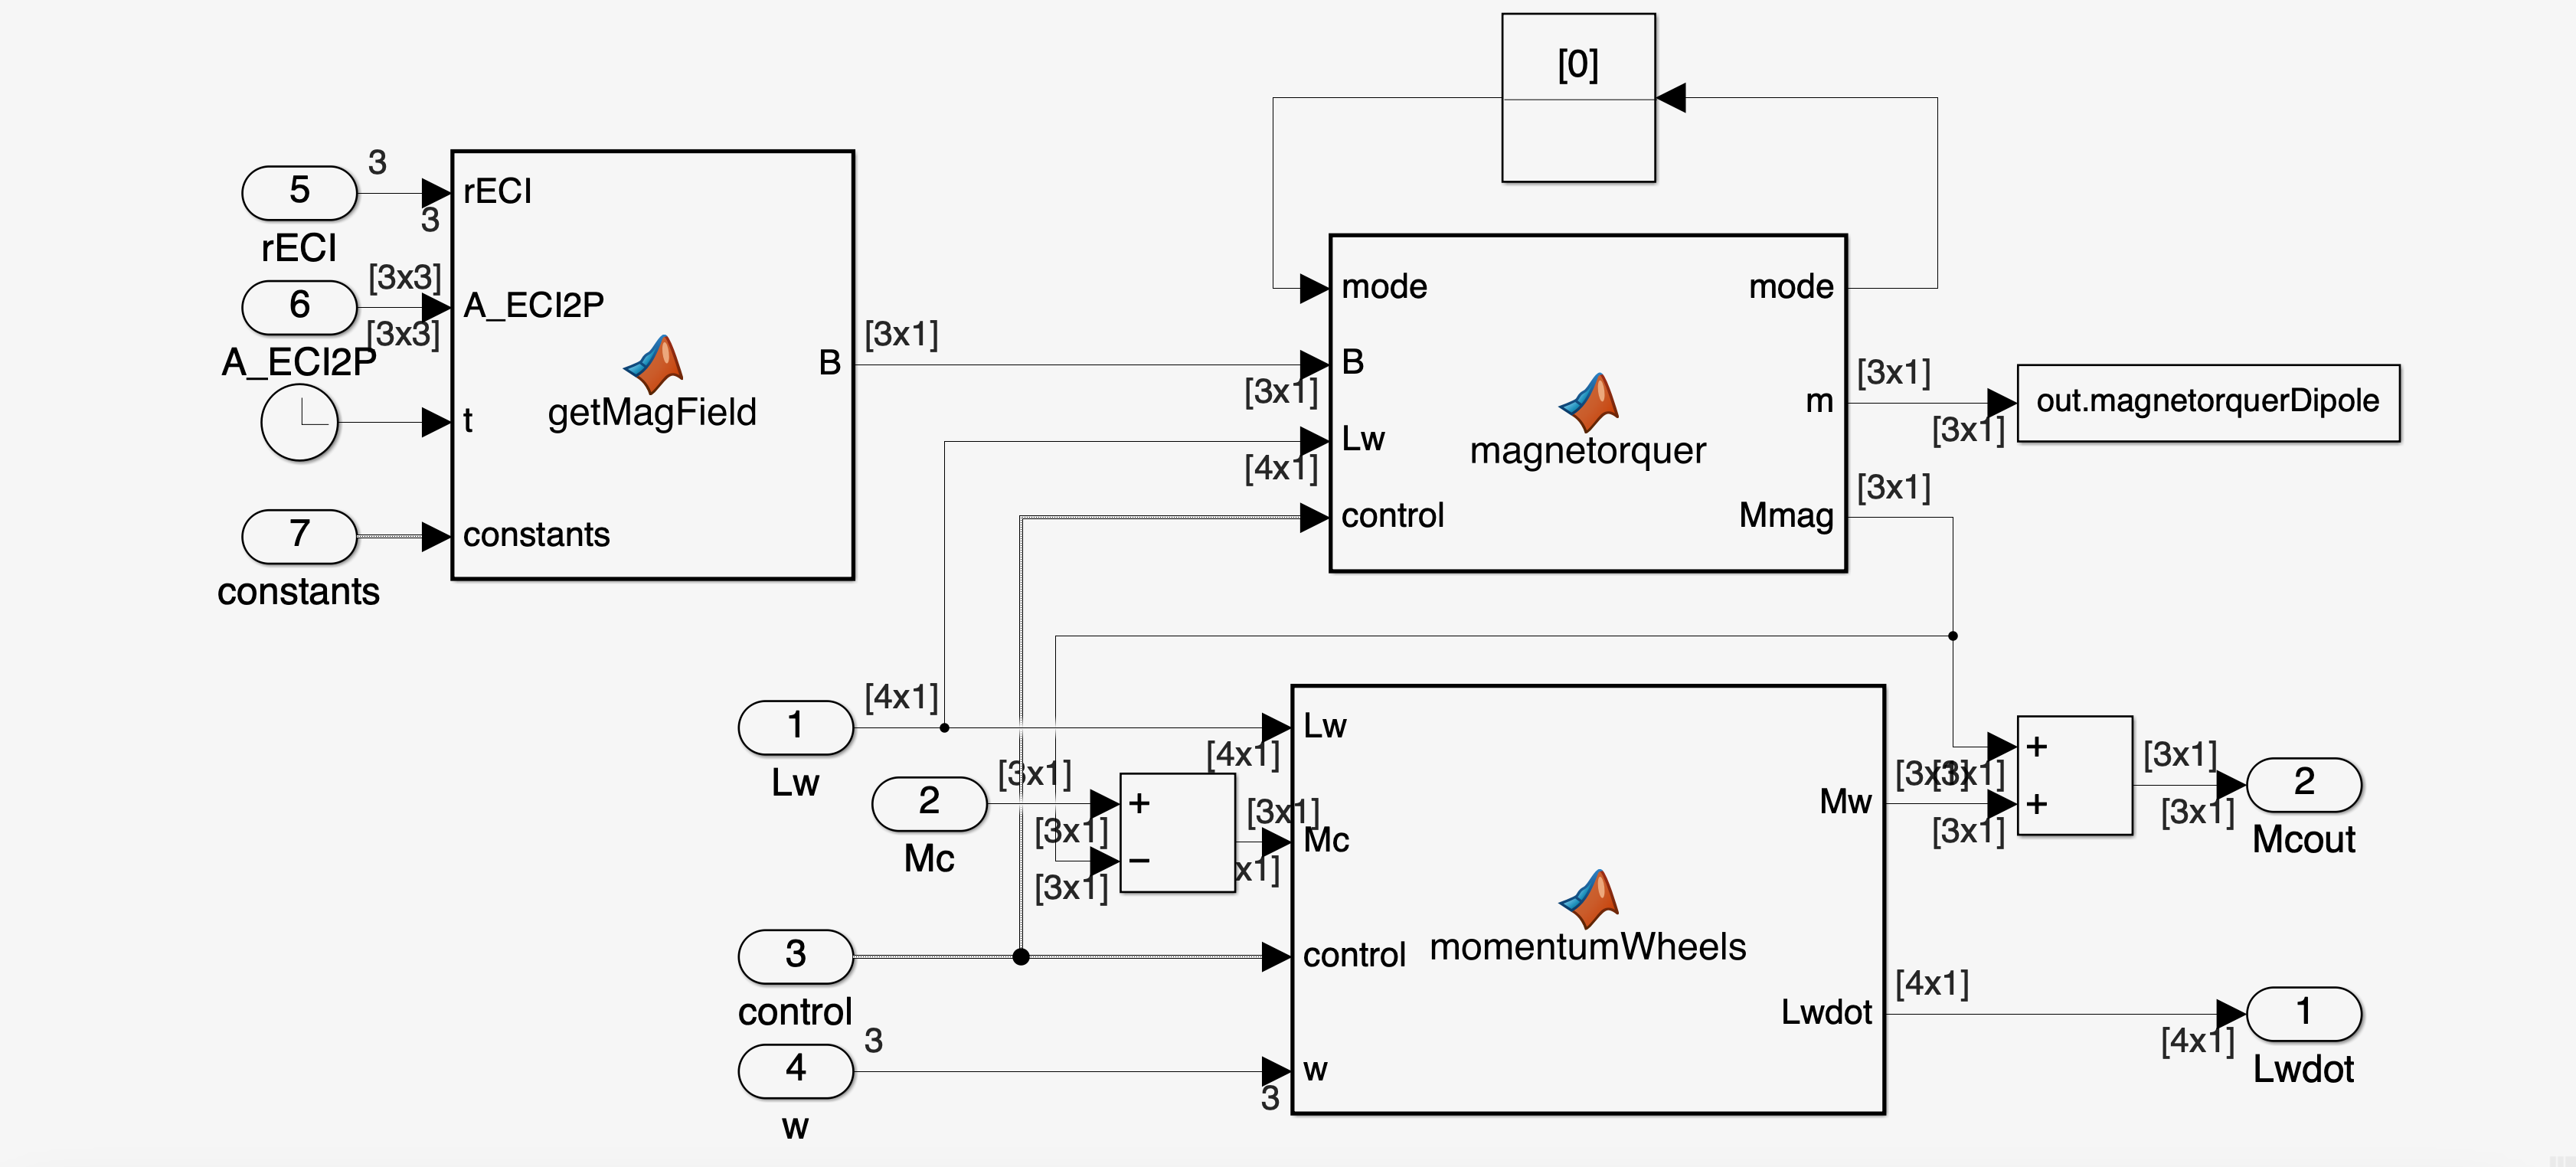
\includegraphics[scale=0.25]{Images/ps10_actuators.png}
\caption{Simulink diagram of actuator subsystem with magnetorquers for desaturation}
\label{fig:ps10_actuators}
\end{figure}

The amount of torque generated can vary at any given moment depending on the attitude of the spacecraft and the location in the magnetic field, which we estimate using a fourth-order model described previously in this paper. For the purpose of desaturation, we assume that the net dipole can be arbitrarily generated based on a 3-axis magnetorquer system.  We assume the commands to individual magnetorquer rods are computed automatically, although we verify that the magnitude of the dipole and resulting torque are realistic in selecting our gain coefficient.

[INSERT DESATURATION MAGNETORQUER EQUATIONS HERE]

In order to generate the desired torque for desaturation, we must determine the direction of the torque which will permit us to slow down the reaction wheels while maintaining the desired attitude. We can compute the appropriate dipole moment for our magnetorquer system based on the net angular momentum vector of our reaction wheel system. The resultant torque can be found as the cross product of this dipole with the magnetic field.

To fully achieve desaturation, we must also include the reaction wheels in the loop–a corresponding command must be sent to the reaction wheels as well. We can achieve this by taking the difference of the original torque command (based on our original attitude error control law) and the torque from the magnetorquer (an estimate which may be based on measurements, although our simulation uses the exact value for simplicity) and sending this as the new torque command to our reaction wheels. We can also neglect to include the magnetorquer torque in the torque command and simply rely on the controller to account for the attitude error, essentially treating the magnetorquer torque as another disturbance (albeit a beneficial one), but this leads to increased attitude control error during desaturation.

Implementing this controller in simulation, we can observe that the desaturation control law using magnetorquers does indeed work to desaturate the reaction wheels. Figure \ref{fig:ps10_angular_velocity} shows that the reaction wheel never saturates, and we require desaturation every 12-14 orbits, or approximately daily.

\begin{figure}[H]
\centering
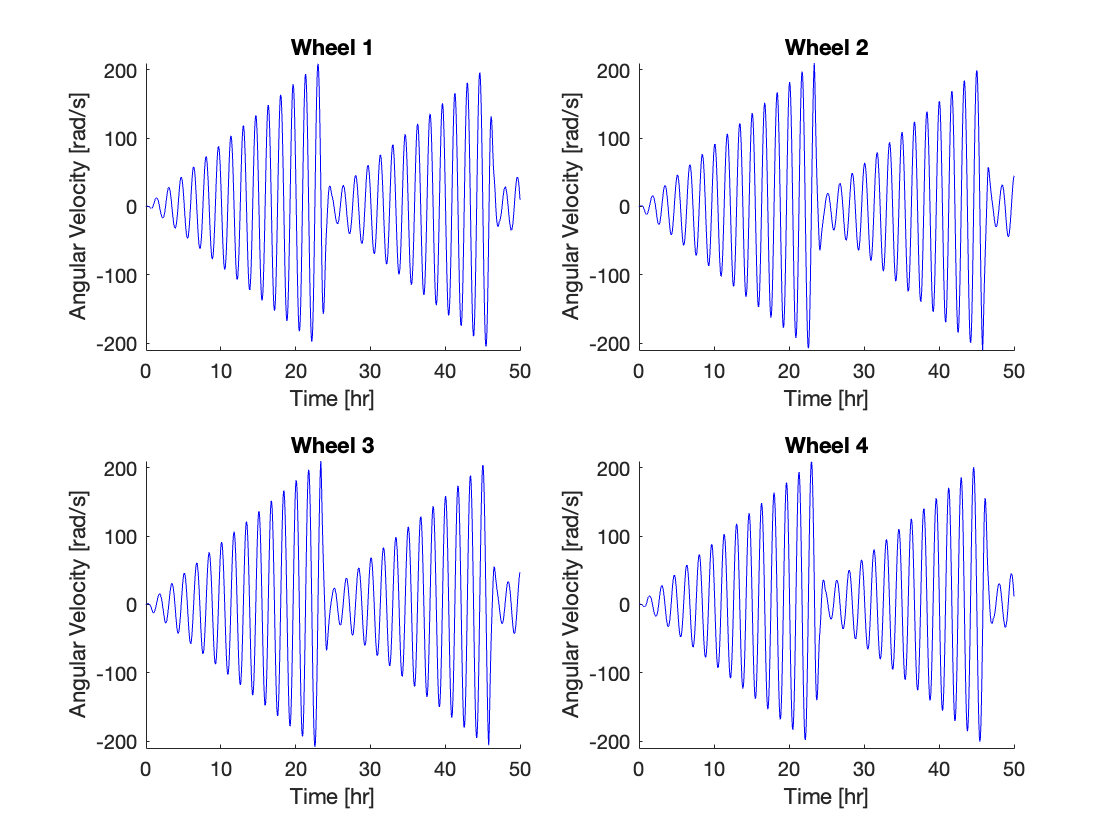
\includegraphics[scale=0.3]{Images/ps10_angular_velocity.png}
\caption{Angular velocity of reaction wheels over 30 orbits}
\label{fig:ps10_angular_velocity}
\end{figure}

In this implementation, our desaturation mode is activated whenever any reaction wheel reaches half of the maximum angular momentum capability and ceases whenever all reaction wheels are desaturated to a tenth of this threshold. Our gain is chosen as $K = 0.001$, on the same order of magnitude as the value ($K = 0.003$) used in Hogan and Schaub \cite{Hogan2015}. Desaturation occurs relatively quickly, and over the course of 30 orbits, only two desaturation periods are required.

\begin{figure}[H]
\centering
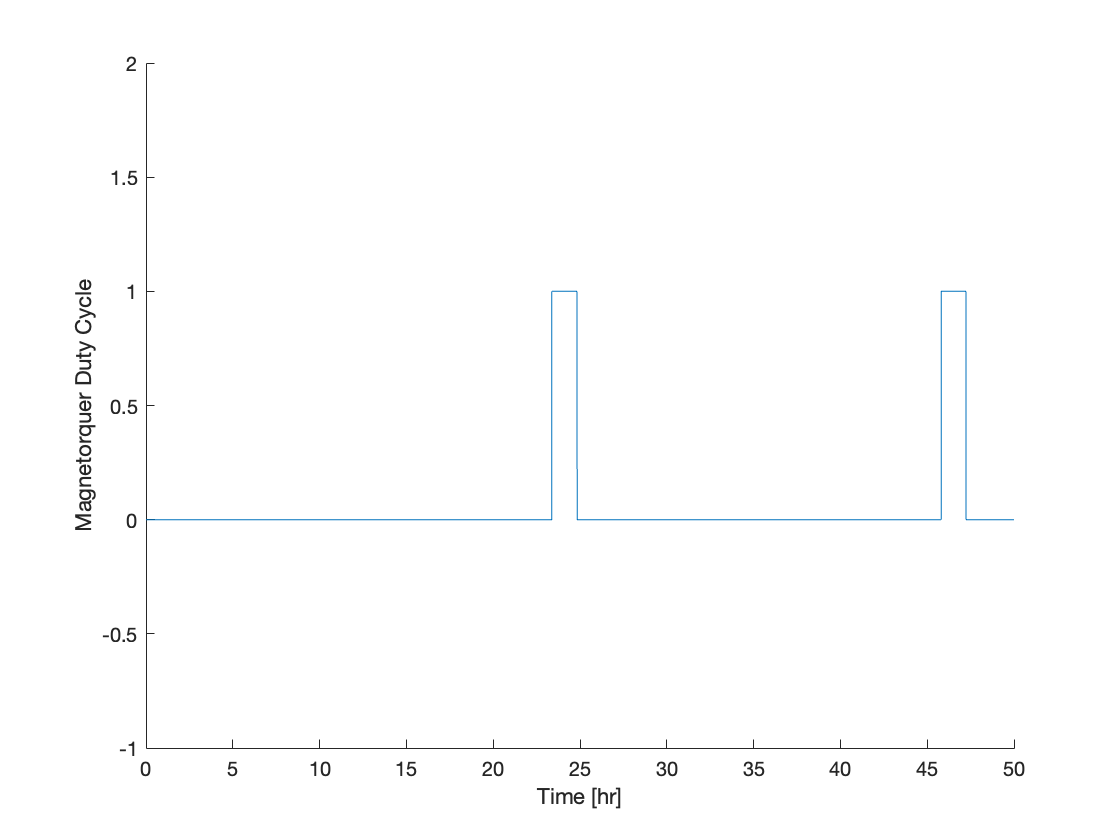
\includegraphics[scale=0.25]{Images/ps10_desaturation_mode.png}
\caption{Desaturation mode over 30 orbits (0 is off, 1 is on)}
\label{fig:ps10_desaturation_mode}
\end{figure}

We also verify that the attitude control error remains within our bounds for the duration of the simulation. Figure \ref{fig:ps10_error_closed_loop} shows attitude control error for the case where our controller accounts for the magnetorquer torque, while Figure \ref{fig:ps10_error_open_loop} shows attitude control error when the magnetorquer is not accounted for.

\begin{figure}[H]
\centering
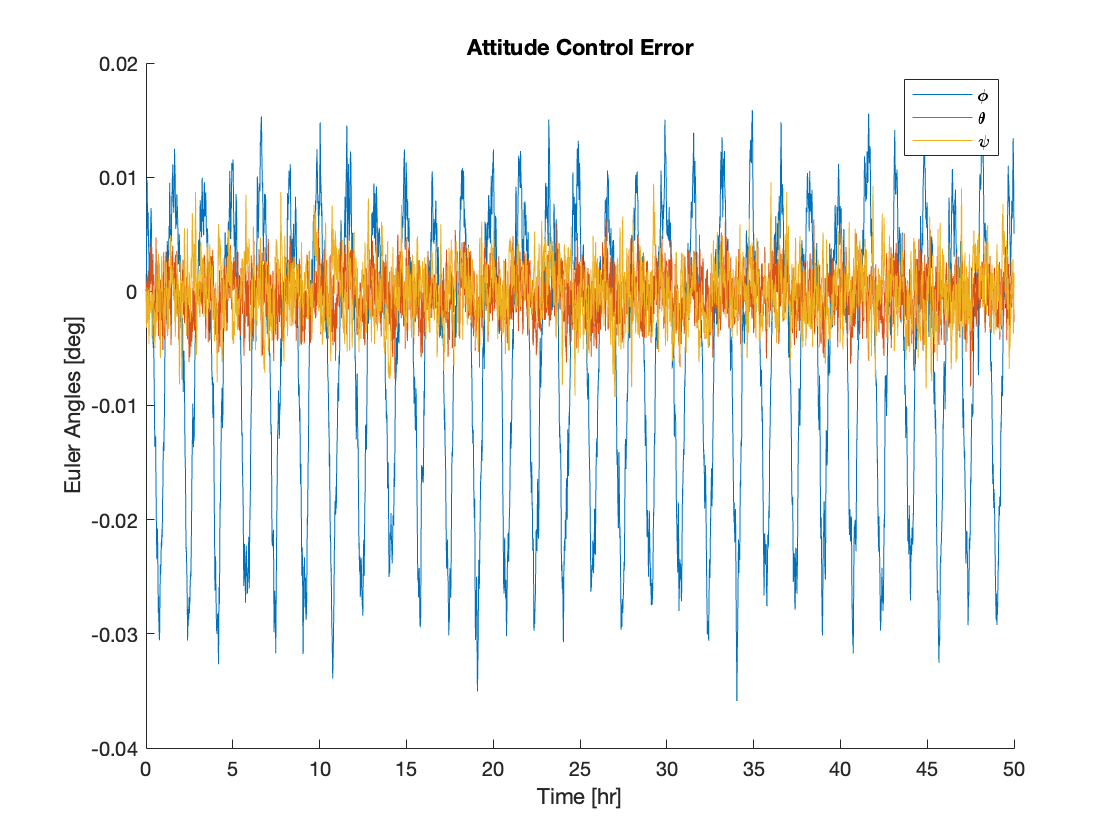
\includegraphics[scale=0.3]{Images/ps10_error_closed_loop.png}
\caption{Attitude control error, considering magnetorquer in reaction wheel command}
\label{fig:ps10_error_closed_loop}
\end{figure}

\begin{figure}[H]
\centering
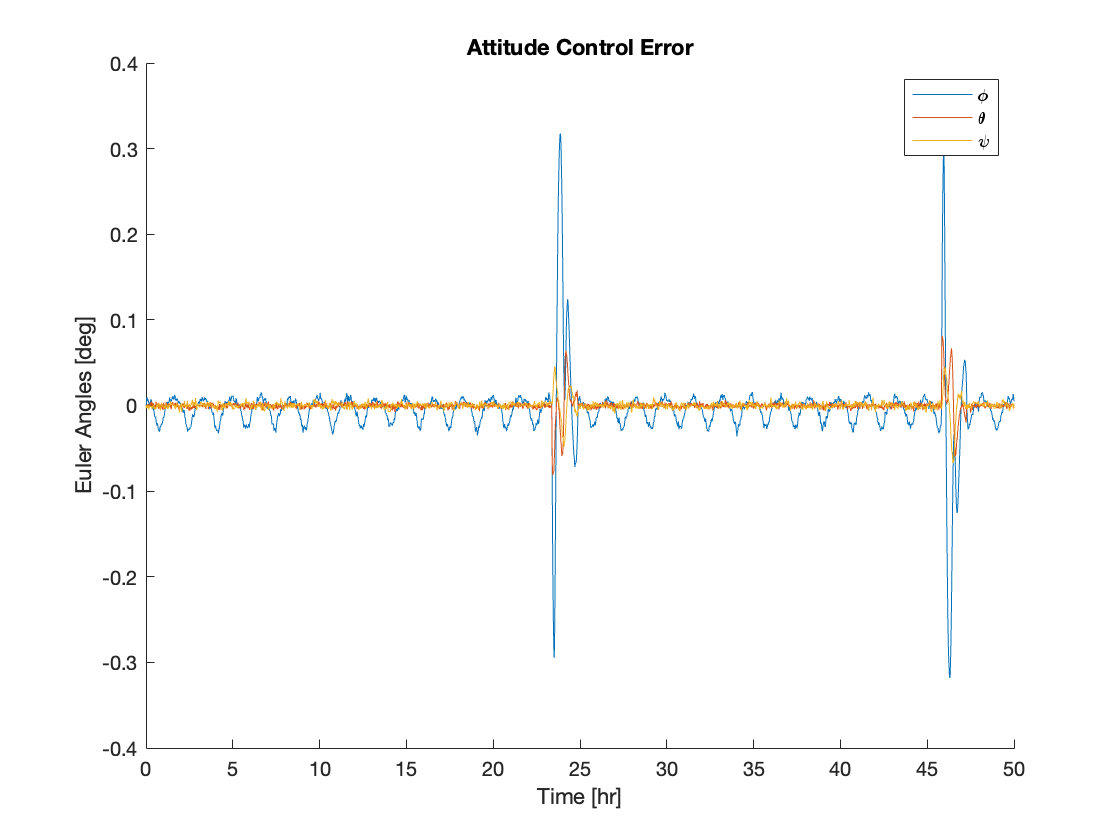
\includegraphics[scale=0.3]{Images/ps10_error_open_loop.png}
\caption{Attitude control error, not modeling for magnetorquer torques}
\label{fig:ps10_error_open_loop}
\end{figure}

The attitude control error remains consistently very low–identical to nominal controller operation in the previous section–as expected for the case where we account for the additional torque. However, if we do not include this additional torque, while attitude control error remains the same as before when magnetorquers are not operating, we observe periods of relatively large attitude control error during desaturation. We can infer from this data that a noisy or inaccurate estimate of the resultant torque from the magnetorquers has an impact on pointing accuracy during magnetorquer operation, but it not enough to destabilize the system, which is able to resume normal pointing accuracy immediately after desaturation is complete. This may be acceptable if no activities requiring precision control are occurring in parallel with desaturation and if the desaturation period is relatively short. Otherwise, feeding an accurate prediction of the magnetorquer torque into the actuator system control input allows us to maintain extremely precise pointing accuracy regardless of operating mode.

Additionally, we show the magnetorquer dipole moment and torque over the duration of the simulation.

\begin{figure}[H]
\centering
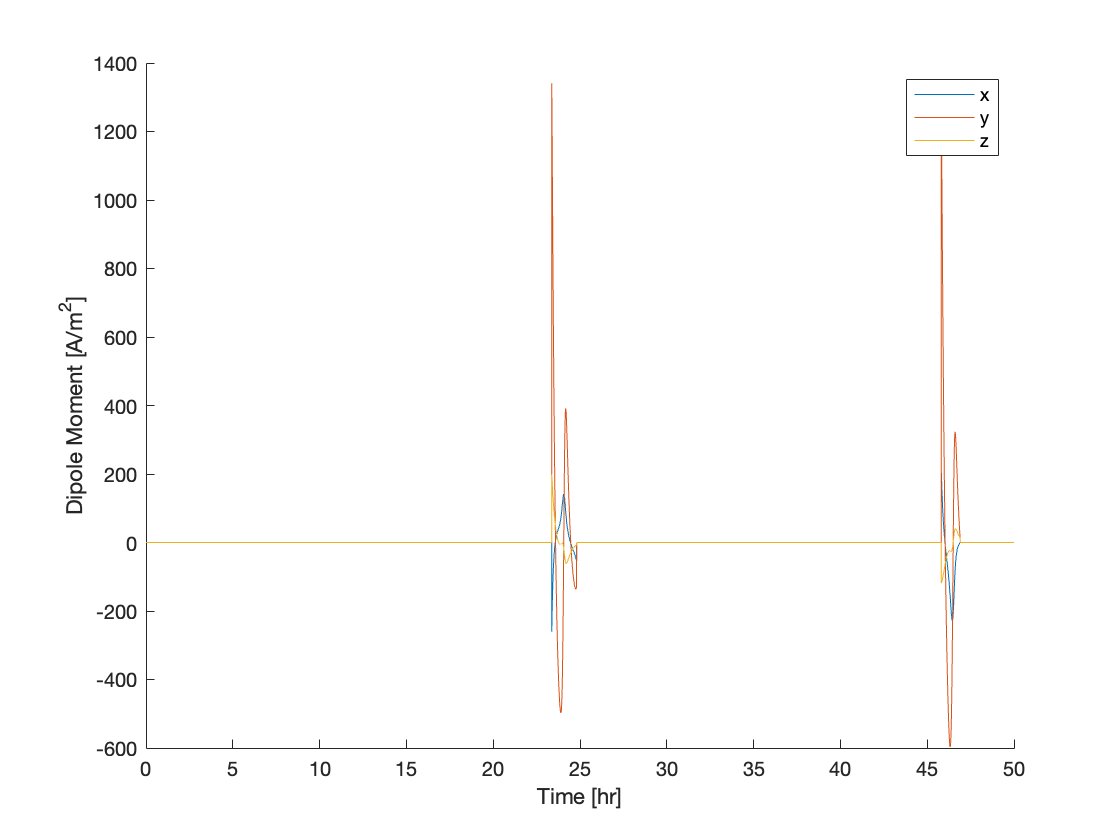
\includegraphics[scale=0.3]{Images/ps10_dipole_moment.png}
\caption{Magnetorquer dipole moments over 30 orbit period}
\label{fig:ps10_dipole_moment}
\end{figure}

\begin{figure}[H]
\centering
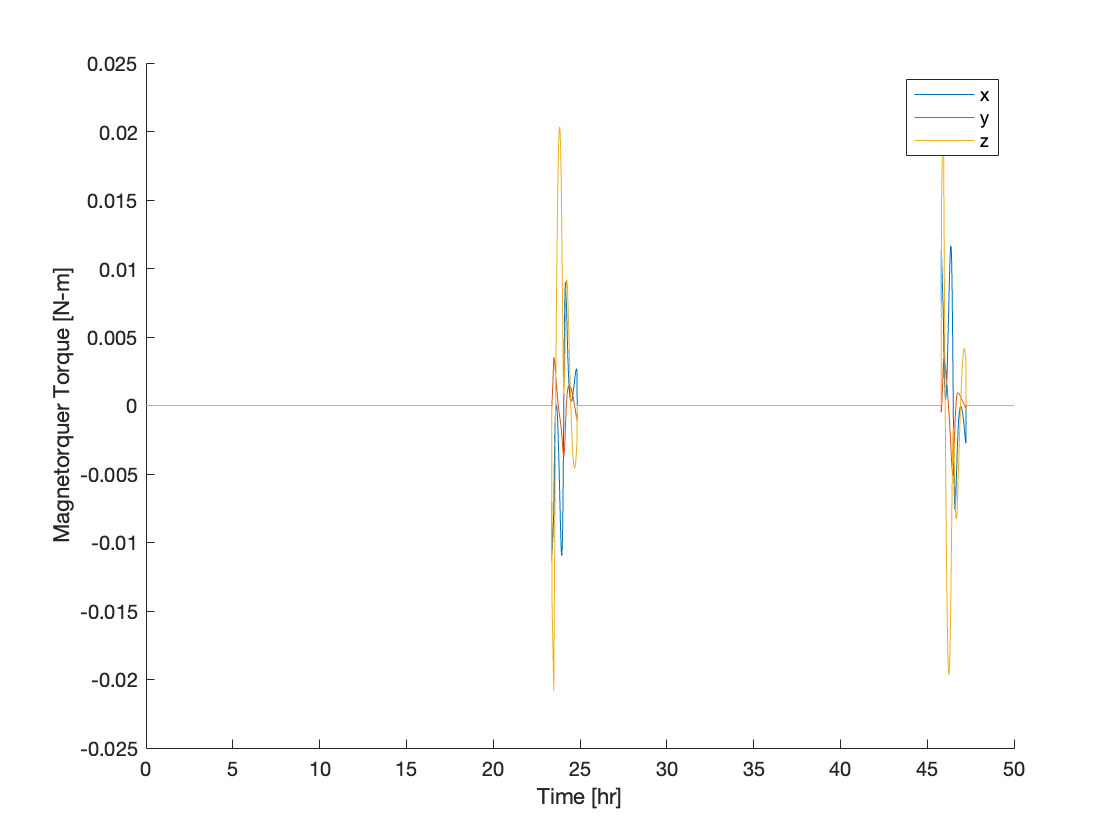
\includegraphics[scale=0.3]{Images/ps10_mag_torque.png}
\caption{Magnetorquer torques over 30 orbit period}
\label{fig:ps10_mag_torque}
\end{figure}

The magnitude of the dipole moment in any axis never exceeds 2000 A/m\textsuperscript{2}, only briefly peaking at approximately 1400 A/m\textsuperscript{2} for short bursts. Most operation does not exceed 500 A/m\textsuperscript{2}. This is a reasonable value for the dipole moment of a satellite of such size \cite{gibson1971low}. Note that this value is much larger than the dipole required for disturbance rejection, as we are effectively canceling out accumulated momentum from disturbances over a much longer period. If additional information about NISAR's magnetorquers were publicly available, it would be possible to model saturation of the magnetorquers if they were to exceed their maximum dipole capability. The torques generated by the magnetorquers during desaturation are approximately 0.03 N-m or less, which is also appropriate for a satellite of NISAR's size. These results were considered when tuning gain parameter $K$ and resulted in our selected value of 0.001.